\clearpage
\title{Problem 6.1}
\author{}
\date{}
\maketitle

\section*{Problem Description}
Write a code to take two input from user as Binary and multiply them using shifting operation and output the result in binary.

\section*{Tools Used}
\begin{itemize}
    \item emu8086 - 8086 Microprocessor Emulator
    \item MacTeX -\LaTeX  compiler.
    \item VS Code with \LaTeX workshop extension as a text editor.
\end{itemize}

\section*{Process}
\subsection*{Code:}

\begin{multicols}{2}{|}
    \begin{minted}[linenos,breaklines,breakanywhere]{nasm}
DATA SEGMENT
    INA DW ?
    INB DW ?   
    COUNT DB 16
DATA ENDS

CODE SEGMENT
    ASSUME CS:CODE,DS:DATA
    
MAIN PROC
    MOV AX,DATA
    MOV DS,AX    
    
    CALL MULTIPLY
    CALL BIN_OUT
    
    MOV AH, 4CH
    INT 21H
MAIN ENDP
    
MULTIPLY PROC
    CALL BIN_IN
    MOV INA, CX
    CALL BIN_IN
    MOV INB, CX
    
    MOV AX, INA
    MOV BX, INB
    PUSH AX
    PUSH BX
    XOR DX, DX
    
    LOOP_:
        TEST BX, 1
        JZ END_IF
        
        ADD DX, AX
        
    END_IF:
        SHL AX, 1
        SHR BX, 1
        
        JNZ LOOP_
        POP AX
        POP BX
        
        RET           
MULTIPLY ENDP

BIN_IN PROC
    XOR BX, BX
    MOV AH, 1
    INT 21H  
        
    INPUT:
        CMP AL, 0DH
        JE EXIT_
        
        AND AL, 0FH
        SHL BX, 1
        OR BL, AL
        
        INT 21H       
        JMP INPUT
        
    EXIT_:
        MOV DL, 0DH
        MOV AH, 2
        INT 21H
        MOV DL, 0AH
        INT 21H
        
        MOV CX, BX
        RET       
BIN_IN ENDP 

BIN_OUT PROC
    MOV BX, DX
        
    PRINT:
            RCL BX, 1
            JC PRINT1
            JNC PRINT0
            
    PRINT1:
        CMP COUNT, 0
        JE END_
            
        MOV DL, '1'
        MOV AH, 2
        INT 21H
        DEC COUNT
        JMP PRINT
            
    PRINT0:
        CMP COUNT, 0
        JE END_ 
            
        MOV DL, '0'
        MOV AH, 2
        INT 21H
        DEC COUNT
        JMP PRINT
        
    END_:
        RET            
            
BIN_OUT ENDP

END MAIN
    \end{minted}
\end{multicols}


\subsection*{Output}
\begin{center}
    \centering
    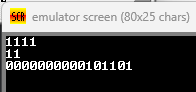
\includegraphics[width = .4\textwidth]{MUL.png}
    \captionof{figure}{Binary input \& output}
\end{center}

